% Figure 1: the matched native round trip, step by step (p50, ns, log scale).
% Data: research-plan.md M1, M3-M8, M11, M12; seL4 from M14.
% Bars in grey were measured with the histogram p50 (before 3349682db).
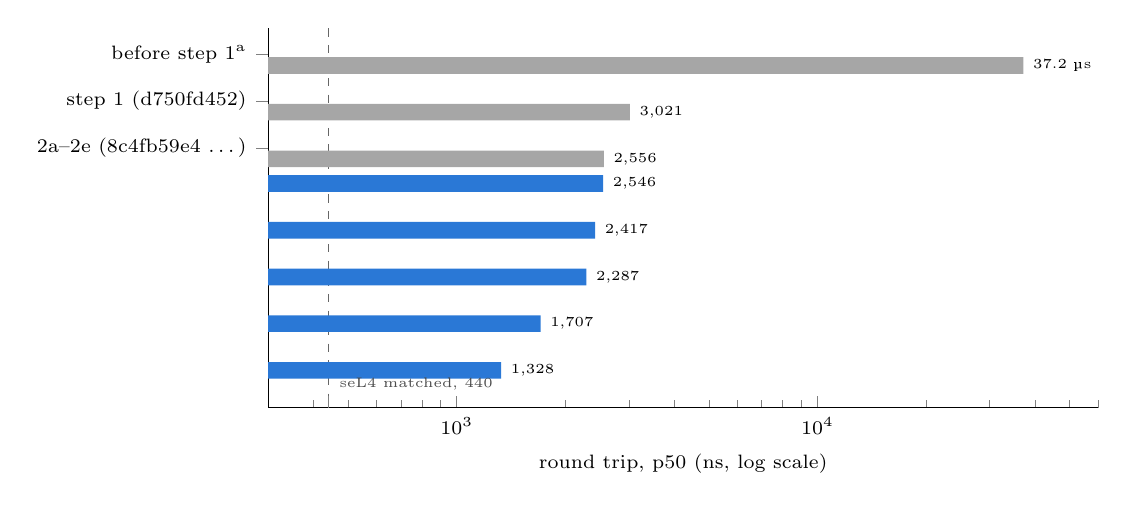
\begin{tikzpicture}
\begin{axis}[
  width=\columnwidth, height=6.4cm,
  xbar, bar width=6pt, xmode=log, xmin=300, xmax=60000,
  log basis x=10,
  xlabel={round trip, p50 (ns, log scale)},
  ytick=data, y dir=reverse,
  yticklabels={
    {before step 1\textsuperscript{a}},
    {step 1 (d750fd452)},
    {2a--2e (8c4fb59e4 \ldots)},
    {exact bench (3349682db)},
    {2f (445d09420)},
    {3a, 3b (a1d456820)},
    {timer, division\textsuperscript{b}},
    {step 4 fast path\textsuperscript{b}}},
  yticklabel style={font=\scriptsize},
  xticklabel style={font=\scriptsize}, xlabel style={font=\scriptsize},
  nodes near coords, nodes near coords style={font=\tiny, anchor=west},
  point meta=explicit symbolic,
  axis x line*=bottom, axis y line*=left,
  enlarge y limits=0.08,
  extra x ticks={440}, extra x tick labels={},
  extra x tick style={grid=major, major grid style={dashed, black!60}},
]
\addplot[fill=black!35, draw=none] coordinates {
  (37191,0) [37.2 µs] (3021,1) [3,021] (2556,2) [2,556] };
\addplot[fill={rgb,255:red,42;green,120;blue,214}, draw=none] coordinates {
  (2546,3) [2,546] (2417,4) [2,417] (2287,5) [2,287] (1707,6) [1,707] (1328,7) [1,328] };
\node[font=\tiny, anchor=south west, black!70] at (axis cs:445,7.4) {seL4 matched, 440};
\end{axis}
\end{tikzpicture}
